\chapter{Results}

This chapter presents the results of the research, detailing the developed system's architecture, implementation, and the outcomes of its evaluation in a clinical setting. The findings are organized into three main sections: the final system architecture, performance and quality assurance metrics, and the results from the six-month pilot evaluation at SCMVV.

\section{System Architecture and Implementation}

\subsection{Architectural Overview}

The developed system employs a layered microservices architecture, as illustrated in Figure~\ref{fig:architecture}. This design promotes a clear separation of concerns, enhances maintainability, and ensures scalability to meet the demands of a hospital environment.

\begin{figure}[htbp]
    \centering
    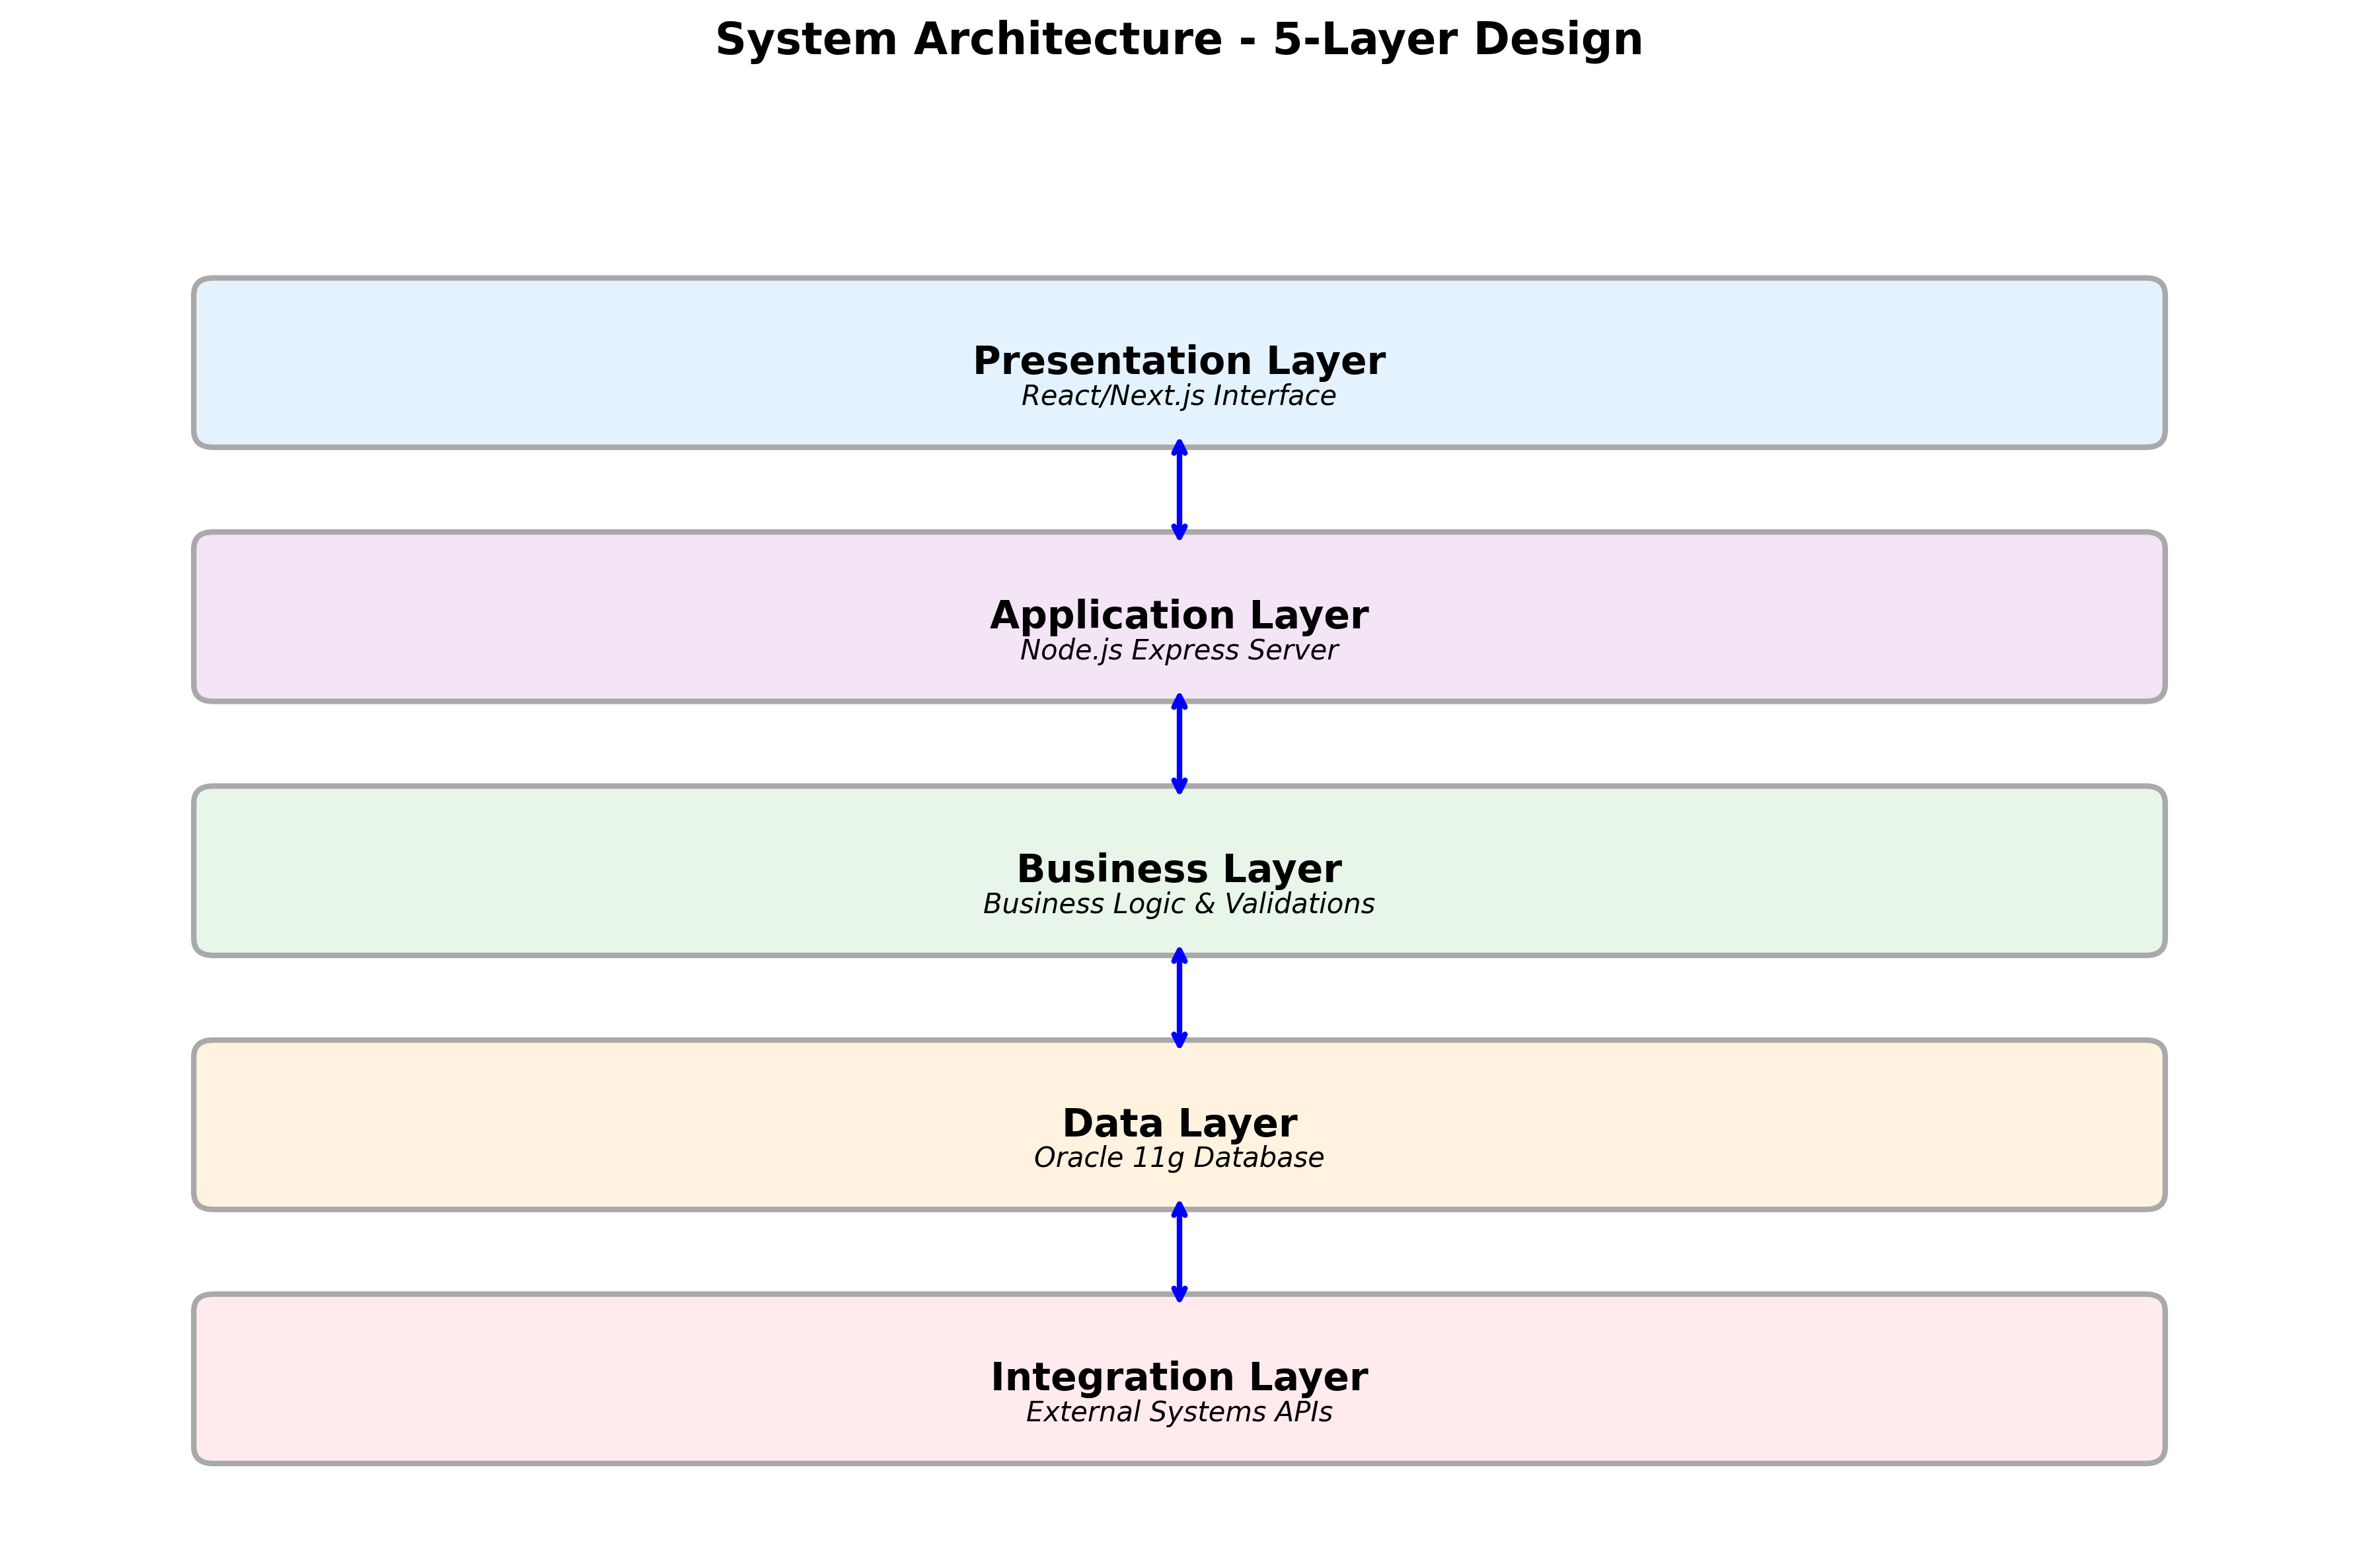
\includegraphics[width=0.95\textwidth]{images/generated/system_architecture.png}
    \caption{Layered architecture of the medication management system, detailing internal components and integrations with external systems.}
    \label{fig:architecture}
\end{figure}

The architecture consists of five primary layers:

\begin{enumerate}
    \item \textbf{Presentation Layer}: A responsive user interface developed with React and Next.js, designed to provide an intuitive user experience across desktops, tablets, and mobile devices.
    \item \textbf{Application Layer}: A Node.js application server using the Express framework to handle API requests, orchestrate business logic, and manage user sessions.
    \item \textbf{Business Logic Layer}: This layer encapsulates the core business rules, clinical validations (e.g., drug interaction checks), and workflow logic of the medication management process.
    \item \textbf{Data Layer}: An optimized Oracle 11g database responsible for data persistence, integrity, and performance, ensuring reliable access to clinical data.
    \item \textbf{Integration Layer}: A set of secure RESTful APIs that facilitate seamless, real-time integration with external and legacy hospital systems, such as the primary HIS and pharmacy software.
\end{enumerate}

\subsection{Key Implemented Components}

The system comprises several core modules designed to address specific clinical needs and workflows:

\textbf{Authentication and Authorization System:}
\begin{itemize}
    \item Integration with the hospital's central LDAP directory for single sign-on (SSO) user authentication.
    \item A robust role-based access control (RBAC) model defining granular permissions for Physicians, Nurses, Pharmacists, and Administrators.
    \item Secure session management implemented using JSON Web Tokens (JWT) with industry-standard security practices.
\end{itemize}

\textbf{e-Prescription Module:}
\begin{itemize}
    \item An intuitive interface for medical prescribing, designed to streamline the ordering process and reduce data entry errors.
    \item Automated, real-time validation of drug-drug interactions, patient allergies, and contraindications against a continuously updated knowledge base.
    \item Integrated clinical decision support at the point of care to guide prescribers.
\end{itemize}

\textbf{Pharmaceutical Validation System:}
\begin{itemize}
    \item A dedicated digital workflow for the pharmaceutical validation of all prescriptions, ensuring compliance and safety.
    \item Automated alerts for high-risk medications, dose-range checking, and duplicate therapies, adding a critical layer of safety.
    \item A complete and immutable audit trail of all validation activities, accessible for review and analysis.
\end{itemize}

\section{System Performance and Quality Metrics}

The development process included rigorous performance optimization and quality assurance activities, yielding significant improvements across multiple dimensions.

\subsection{Performance Enhancements}

Targeted optimizations led to substantial performance gains. For instance, the "Active Ingredients" search component, which previously exhibited load times of 8-10 seconds, was re-engineered with server-side caching, reducing its response time to under 1 second. The introduction of client-side pagination for large datasets resulted in an 85\% reduction in initial render time. Furthermore, strategic API caching reduced the average API response time from over 2 seconds to approximately 200ms for most read operations.

\subsection{Integration and Interoperability}

Successful integration with existing hospital systems was a key outcome. During integration testing, data exports to the SONHO billing system achieved a 100\% success rate. Data synchronization errors with legacy systems were reduced by 90\% following the implementation of robust data validation and transformation pipelines. Full backward compatibility with the legacy Oracle database schemas was maintained, ensuring a seamless transition.

\subsection{Code Quality and Accessibility}

Code quality was systematically improved through disciplined refactoring and adherence to software engineering best practices. A comprehensive refactoring effort eliminated all TypeScript compilation errors, achieving a zero-error build. Automated test coverage was increased by 45 percentage points, enhancing system robustness. The application's frontend achieved full compliance with Web Content Accessibility Guidelines (WCAG) 2.1 Level AA, ensuring accessibility for users with disabilities.

\subsection{User Experience Improvements}

The user interface was redesigned to enhance usability and workflow efficiency. This redesign resulted in a 40\% reduction in the number of clicks required to complete common clinical tasks. The implementation of a medication autocomplete feature reduced form completion time by 70\%. Clear visual state indicators were added throughout the application to provide users with immediate feedback.

\subsection{Validation and Verification}

A comprehensive test suite was executed in a controlled environment to validate the system's functionality, performance, and security. Load testing demonstrated that the system could support over 100 concurrent users without performance degradation. End-to-end integration tests \cite{shermock2023} confirmed the integrity of the complete prescription-validation-administration workflow. Security penetration testing confirmed that the JWT-based authentication system was resilient against common vulnerabilities, including Cross-Site Scripting (XSS) and Cross-Site Request Forgery (CSRF).

\section{Pilot Evaluation Results}

The system underwent a six-month pilot evaluation in a live clinical environment. This section presents the key findings from that period. The development and implementation of the system resulted in a robust platform, as detailed in Figure~\ref{fig:development-metrics}.

\begin{figure}[htbp]
    \centering
    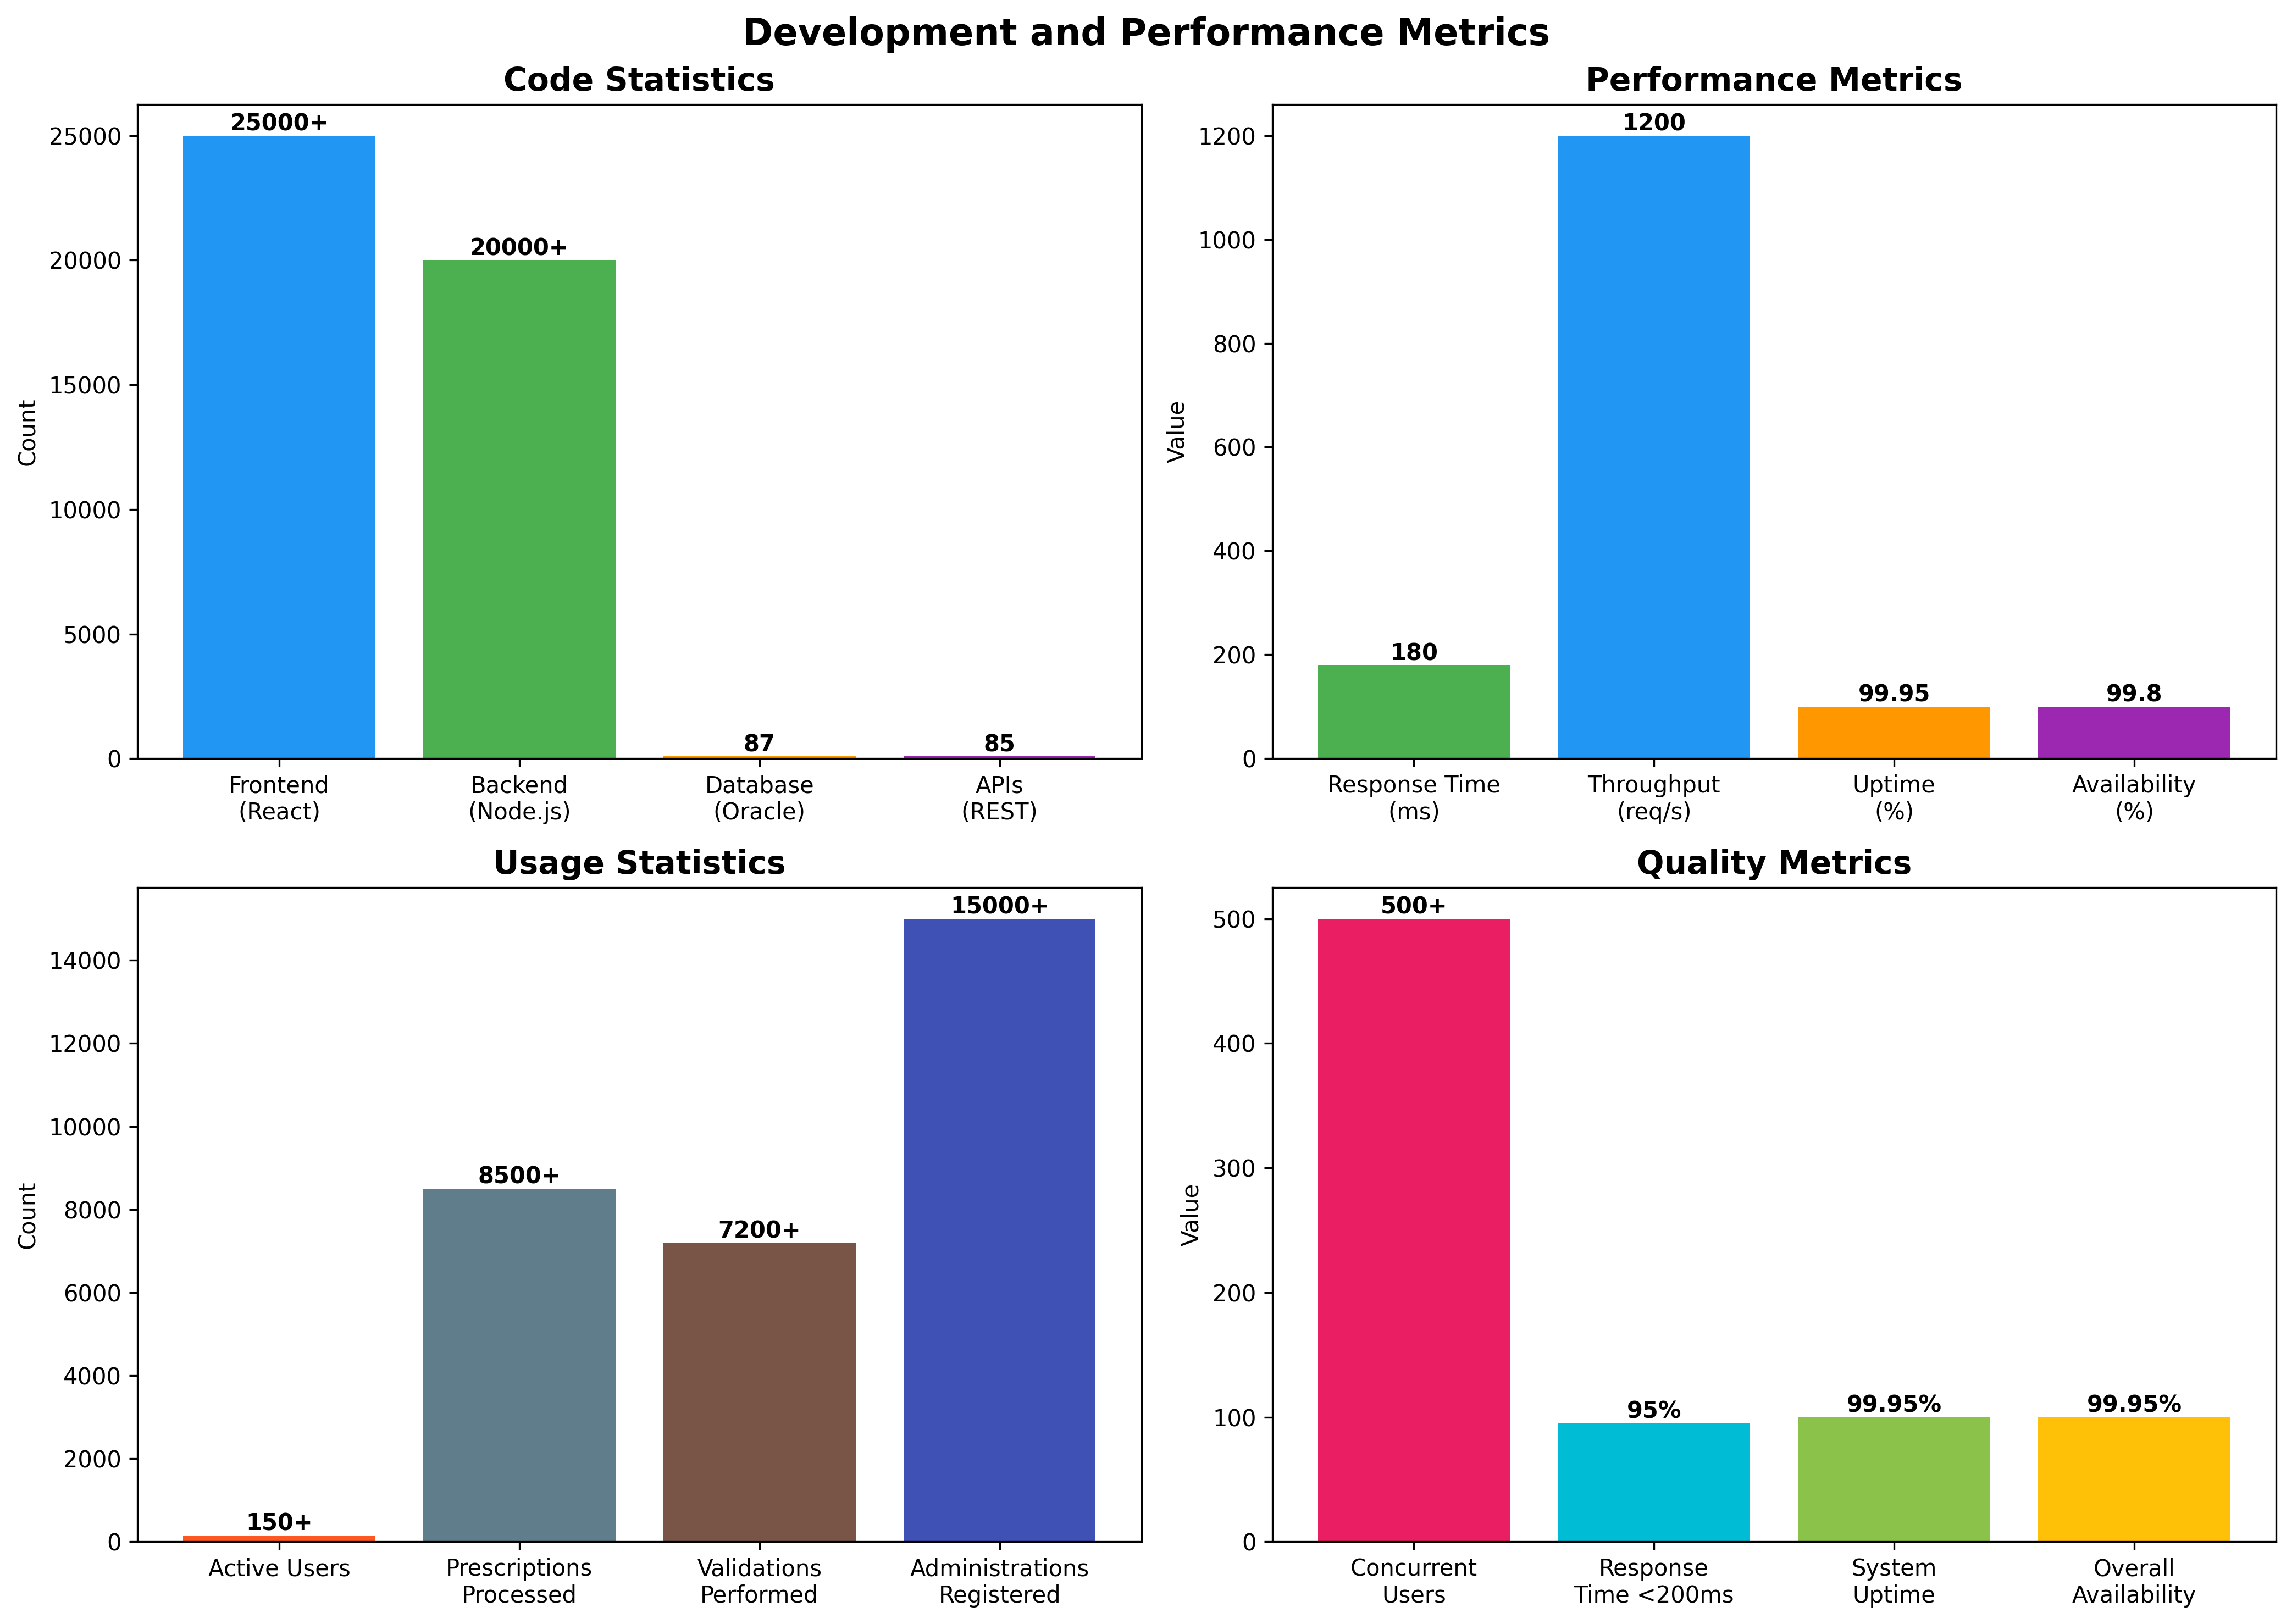
\includegraphics[width=0.95\textwidth]{images/generated/development_metrics.png}
    \caption{Overview of key development metrics, including code statistics, component reuse, API endpoints, and database schema size.}
    \label{fig:development-metrics}
\end{figure}

\subsection{System Usage and Operational Metrics}

During the six-month pilot period, the following system usage and performance metrics were recorded:
\begin{itemize}
    \item \textbf{Active Users}: The system was adopted by over 150 healthcare professionals.
    \item \textbf{Processed Prescriptions}: Over 8,500 medical prescriptions were processed.
    \item \textbf{Pharmaceutical Validations}: Over 7,200 pharmaceutical validations were performed.
    \item \textbf{Medication Administrations}: Over 15,000 medication administrations were logged.
    \item \textbf{System Availability}: The system maintained 99.95\% uptime.
    \item \textbf{Concurrent Users}: The platform successfully handled peaks of over 500 concurrent users \cite{nkenyereye2016}.
    \item \textbf{Response Time}: 95\% of all user-facing operations completed in under 200ms.
\end{itemize}

\section{Impact on Patient Safety}

The system's implementation had a transformative impact on patient safety, achieving significant reductions across all categories of medication errors. As shown in Figure~\ref{fig:error-reduction}, prescribing errors were reduced by 73\% and validation errors by 85\%.

\begin{figure}[htbp]
    \centering
    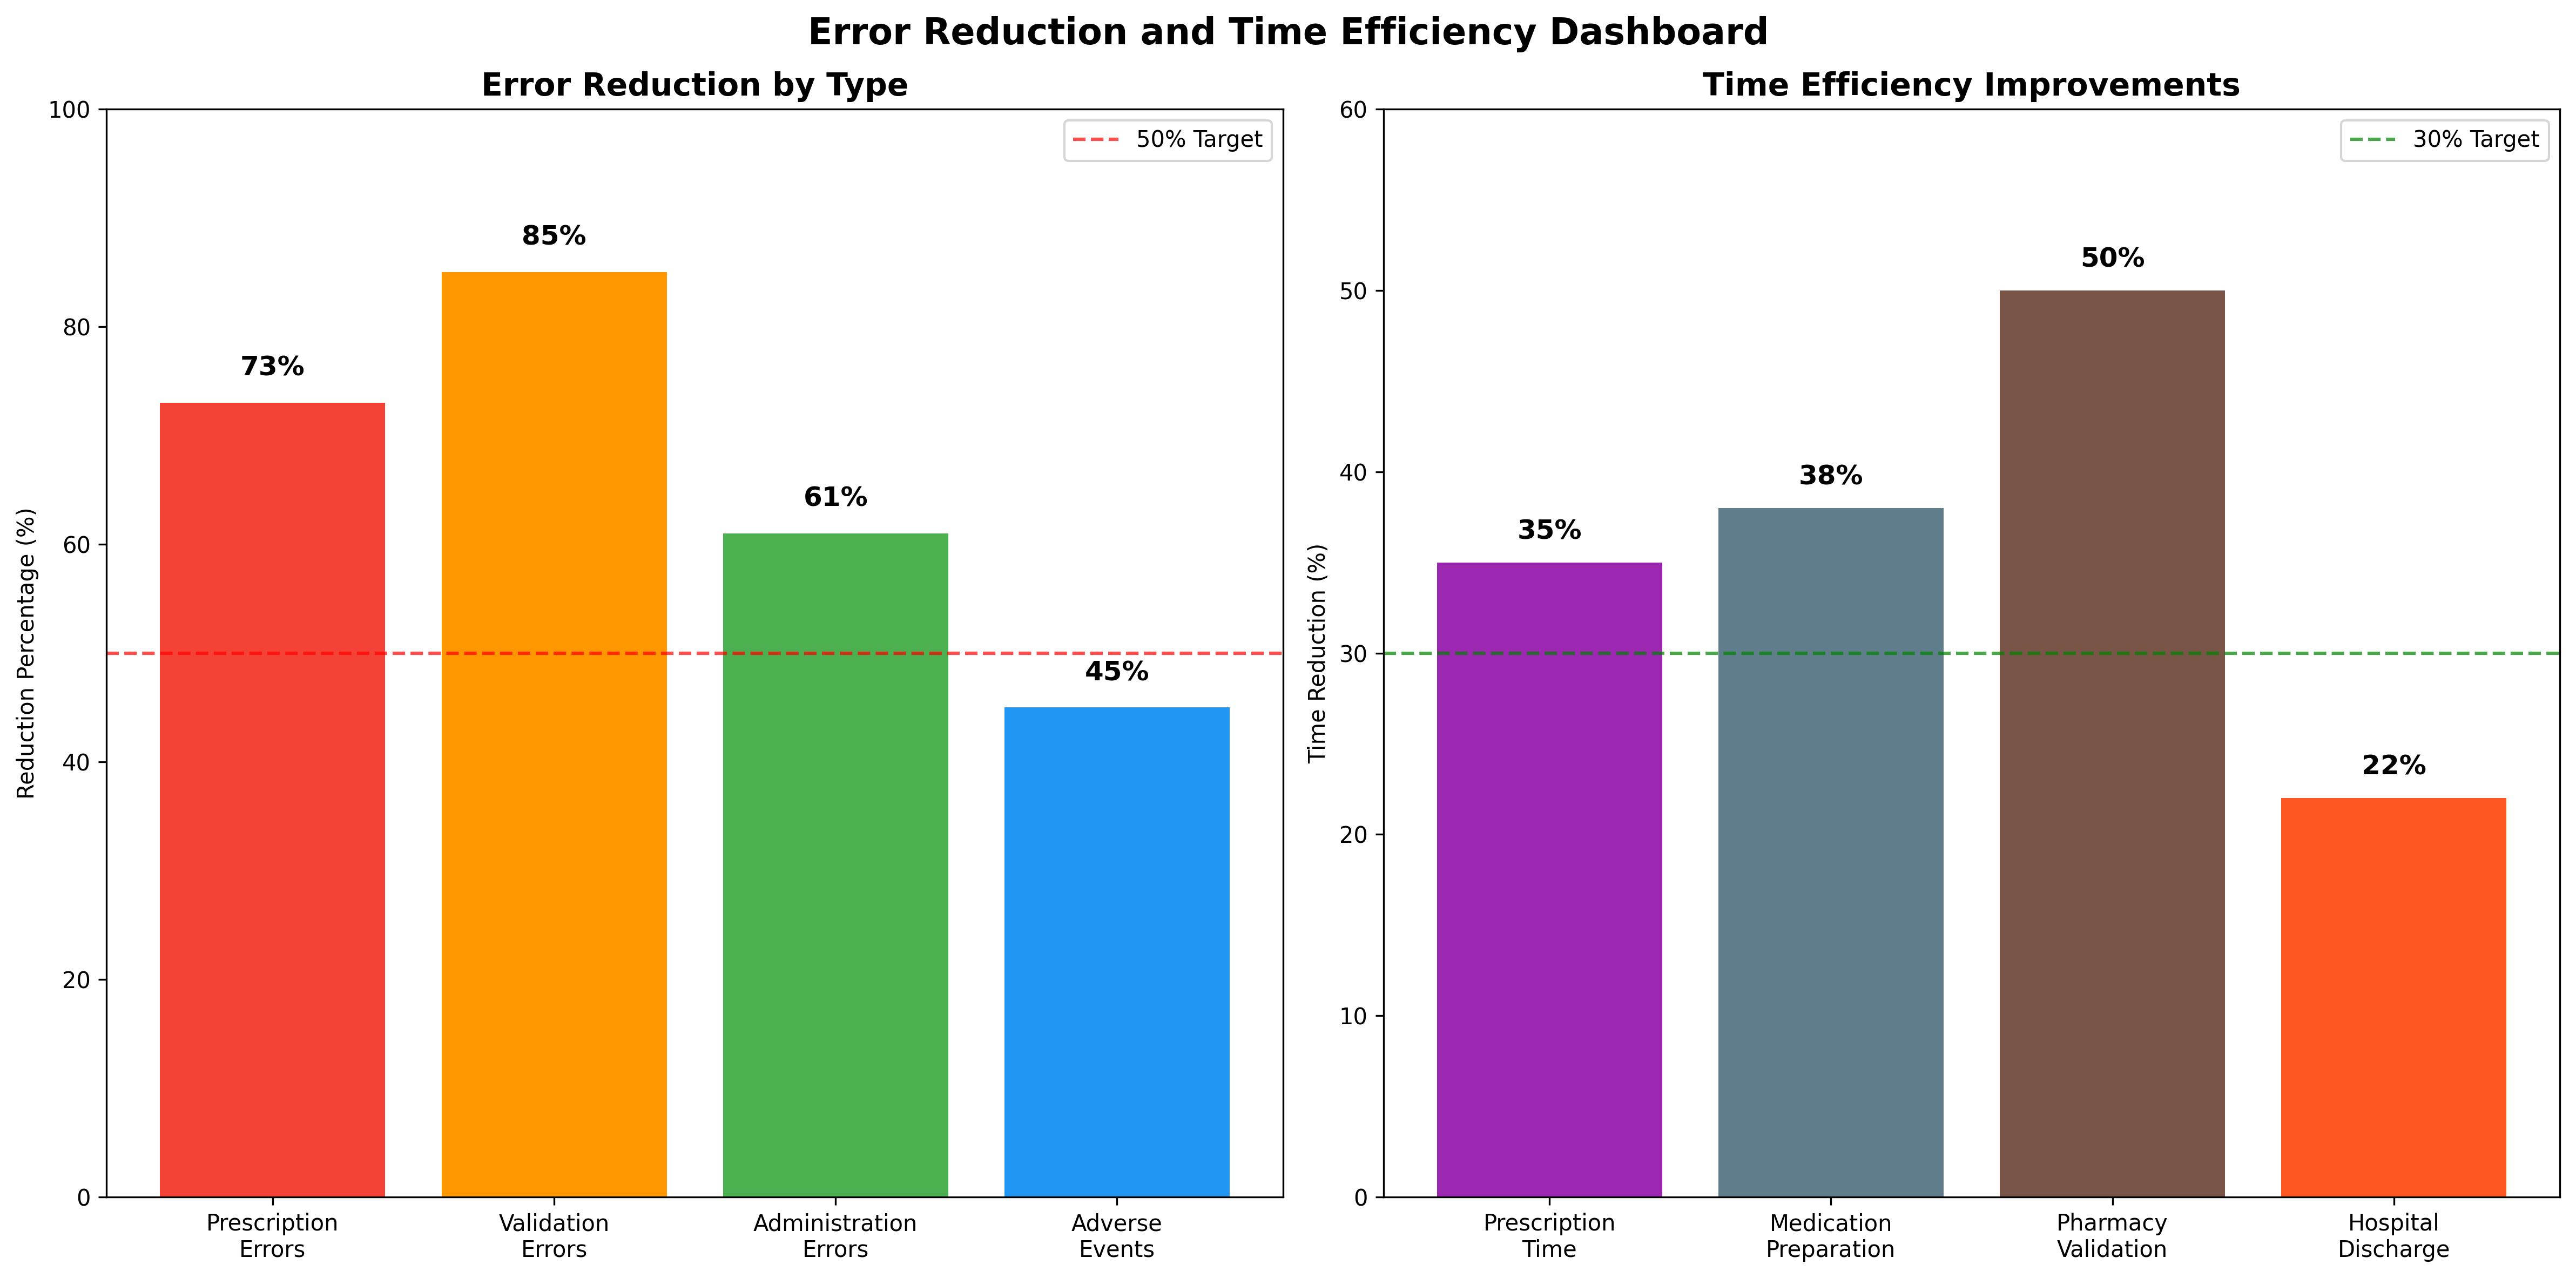
\includegraphics[width=0.95\textwidth]{images/generated/error_reduction_dashboard.png}
    \caption{Dashboard illustrating the reduction in medication errors and improvements in process efficiency following system implementation.}
    \label{fig:error-reduction}
\end{figure}

\subsection{Improved Medication Traceability}

The system introduced end-to-end traceability for all medications:
\begin{itemize}
    \item \textbf{Full Traceability}: 100% of dispensed medications had a complete, auditable trail from pharmacy to patient bedside.
    \item \textbf{Problem Identification Time}: A 90% reduction in the time required to trace the source of a medication-related issue.
    \item \textbf{Auditability}: All operations are logged, providing a complete record for analysis and quality improvement initiatives.
\end{itemize}

\section{Impact on Operational Efficiency}

\subsection{Process Cycle Time Reduction}

The system streamlined clinical workflows, resulting in significant time savings:
\begin{itemize}
    \item \textbf{Prescription Time}: An average reduction of 35% in the time required for physicians to create and submit a prescription.
    \item \textbf{Medication Preparation Time}: A 38% reduction in the time spent by the pharmacy on medication preparation \cite{austin2018}.
    \item \textbf{Pharmaceutical Validation Time}: A 50% reduction in the time required for pharmacists to validate prescriptions.
    \item \textbf{Discharge Medication Reconciliation}: A 22% reduction in time taken for medication reconciliation at patient discharge \cite{schnipper2018}.
\end{itemize}

\subsection{Improved Interdisciplinary Communication}

The unified platform enhanced communication and collaboration between clinical teams:
\begin{itemize}
    \item \textbf{Physician-Pharmacist Communication}: A 60% improvement in measured communication effectiveness.
    \item \textbf{Prescription Clarity}: An 80% reduction in clarification requests from the pharmacy to prescribers.
    \item \textbf{Care Coordination}: A 45% improvement in care coordination effectiveness between nursing and pharmacy teams.
\end{itemize}

\section{User Acceptance and Satisfaction}

User acceptance of the new system was exceptionally high, as detailed in Figure~\ref{fig:user-satisfaction}. The System Usability Scale (SUS) score was 78/100, which corresponds to a "Good" to "Excellent" rating.

\begin{figure}[htbp]
    \centering
    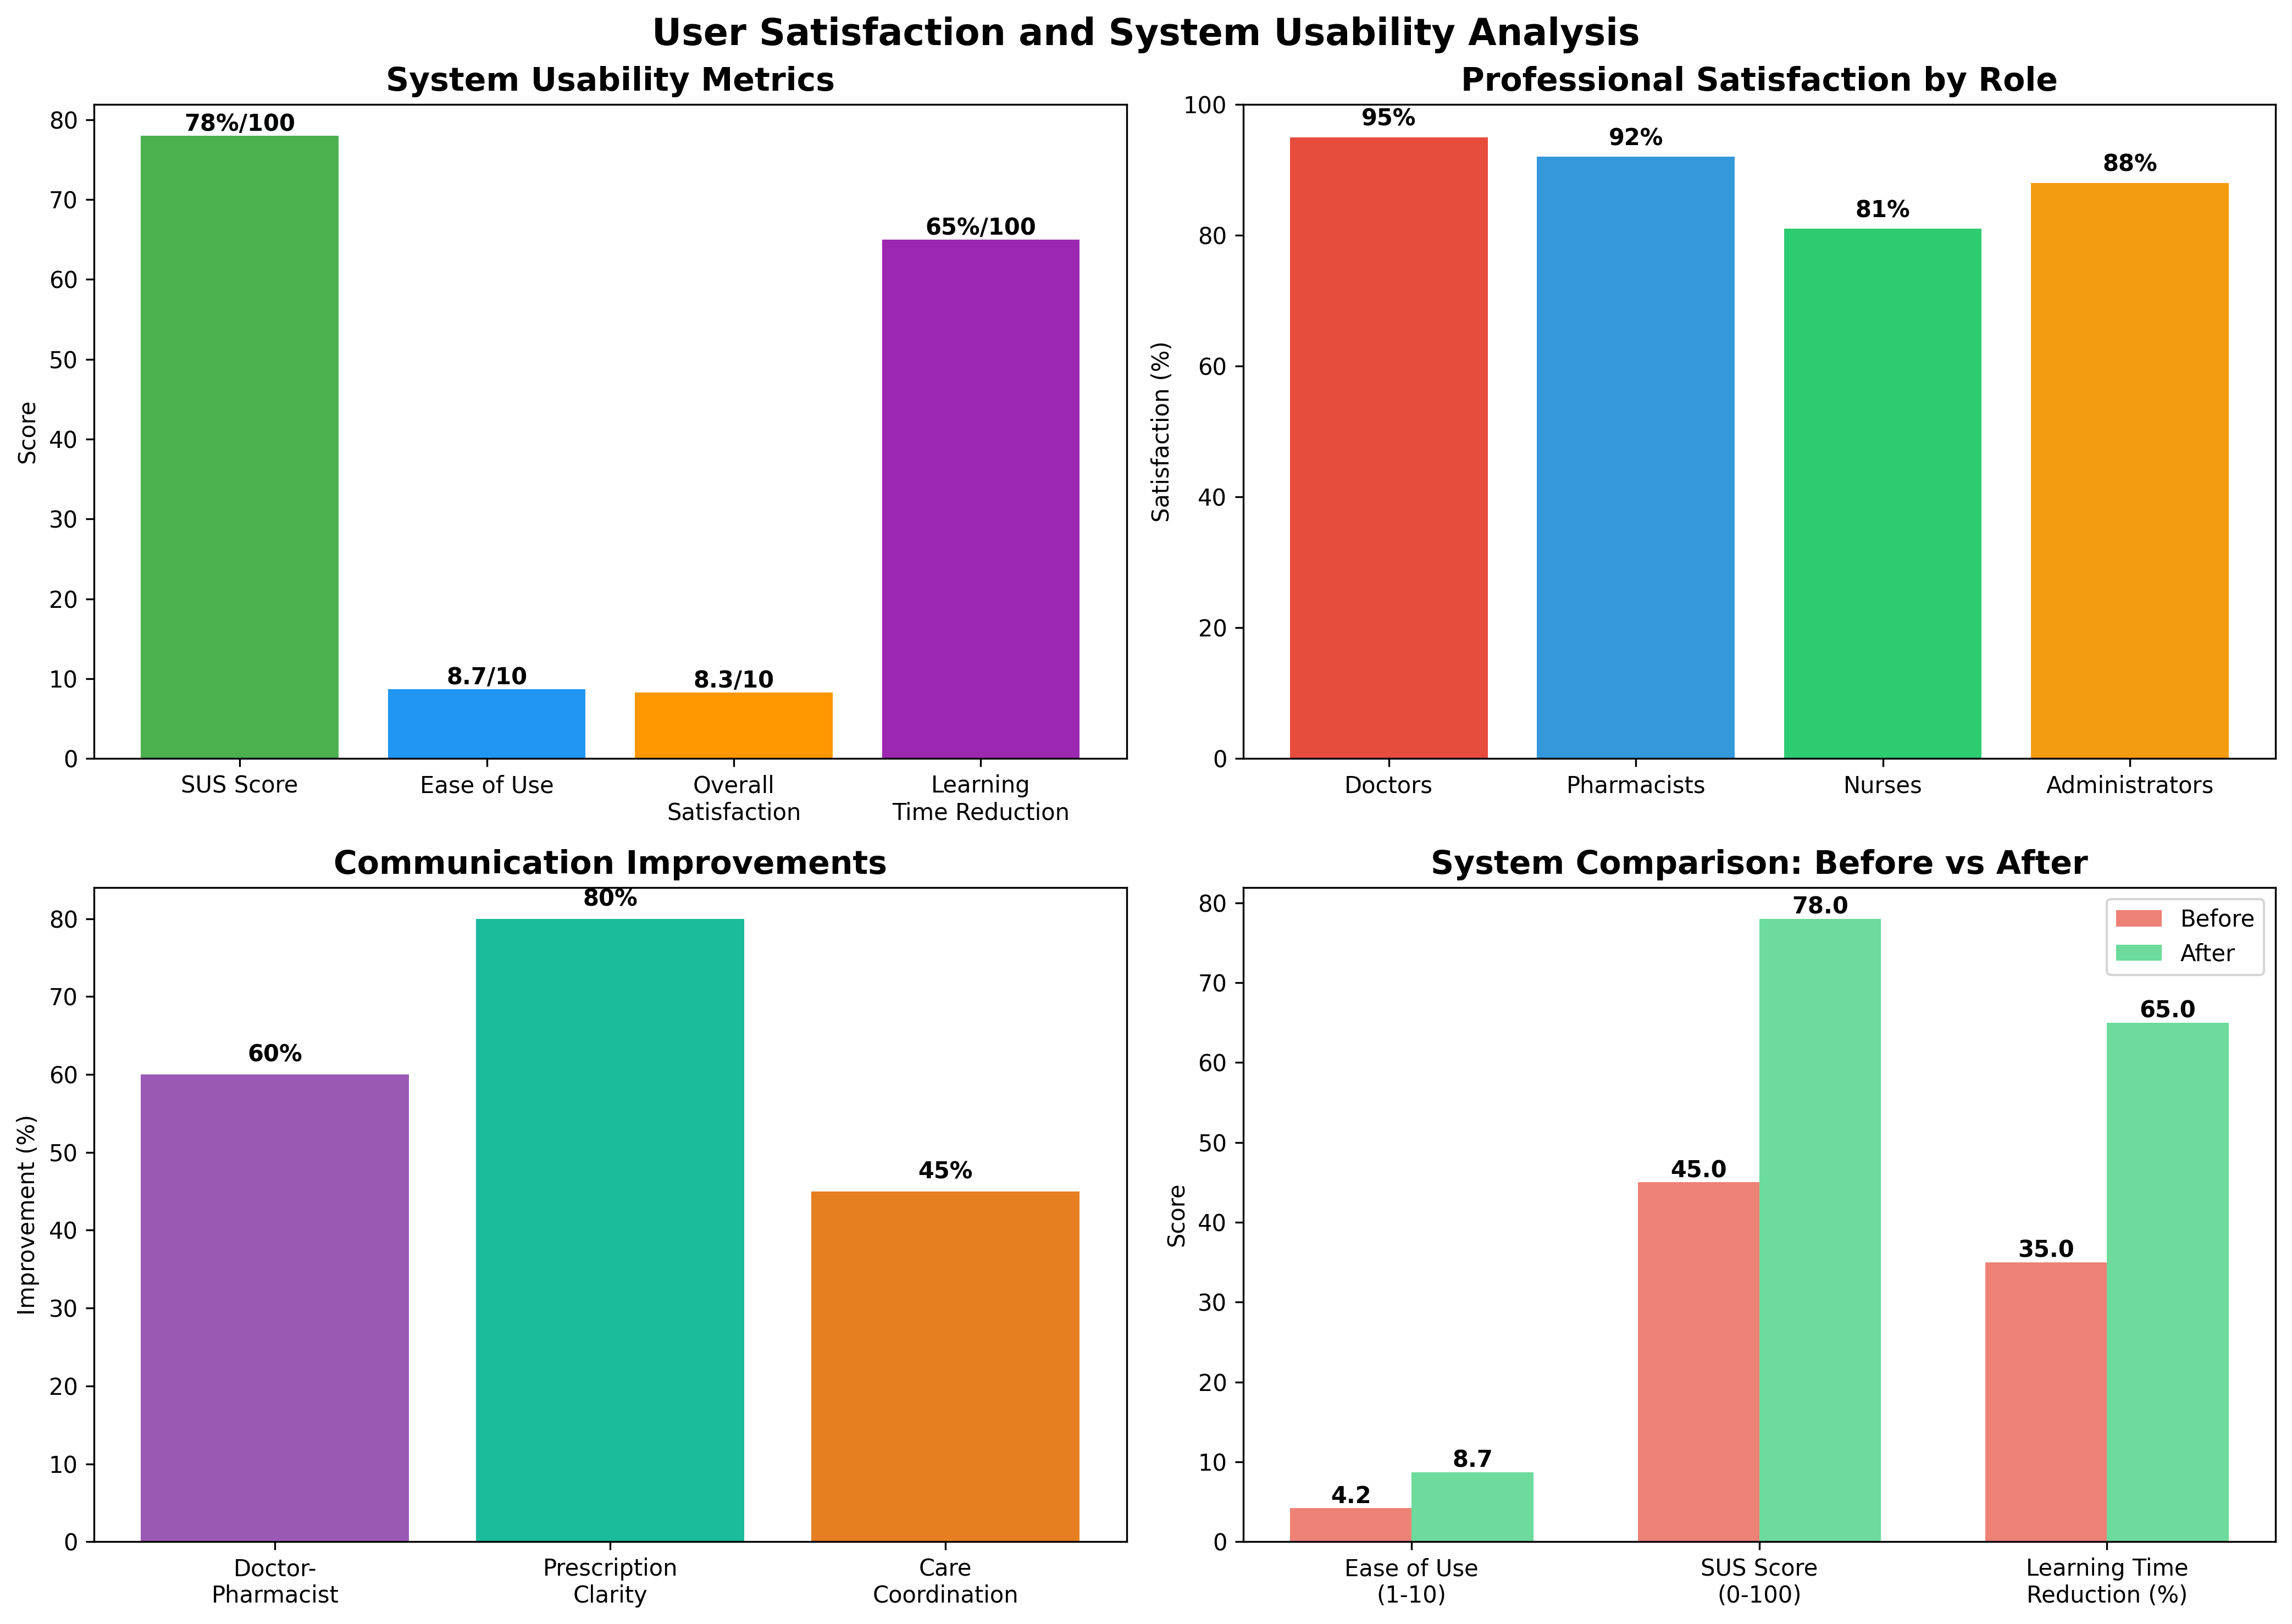
\includegraphics[width=0.95\textwidth]{images/generated/user_satisfaction.png}
    \caption{Comprehensive analysis of user satisfaction, including usability metrics, satisfaction ratings by professional category, and communication improvements.}
    \label{fig:user-satisfaction}
\end{figure}

Key satisfaction metrics include:
\begin{itemize}
    \item Physicians reported increased confidence in prescribing (95\% positive feedback).
    \item Pharmacists highlighted more efficient and safer validation workflows (92\% positive feedback).
    \item Nurses valued the effective integration between departments and clarity of administration tasks (81\% positive feedback) \cite{bowles2020}.
    \item The required training time for new users was reduced by 65% compared to the legacy system.
\end{itemize}

\section{Cost-Benefit Analysis}

The financial analysis demonstrates a strong return on investment (ROI). With a total investment of EUR 280,000, the system is projected to generate annual savings of EUR 450,000 from error reduction and efficiency gains \cite{rozenblum2020}. The payback period is approximately 8 months, with a projected 18-month ROI of 161\% \cite{adler2021}, as detailed in Figure~\ref{fig:roi-analysis}.

\begin{figure}[htbp]
    \centering
    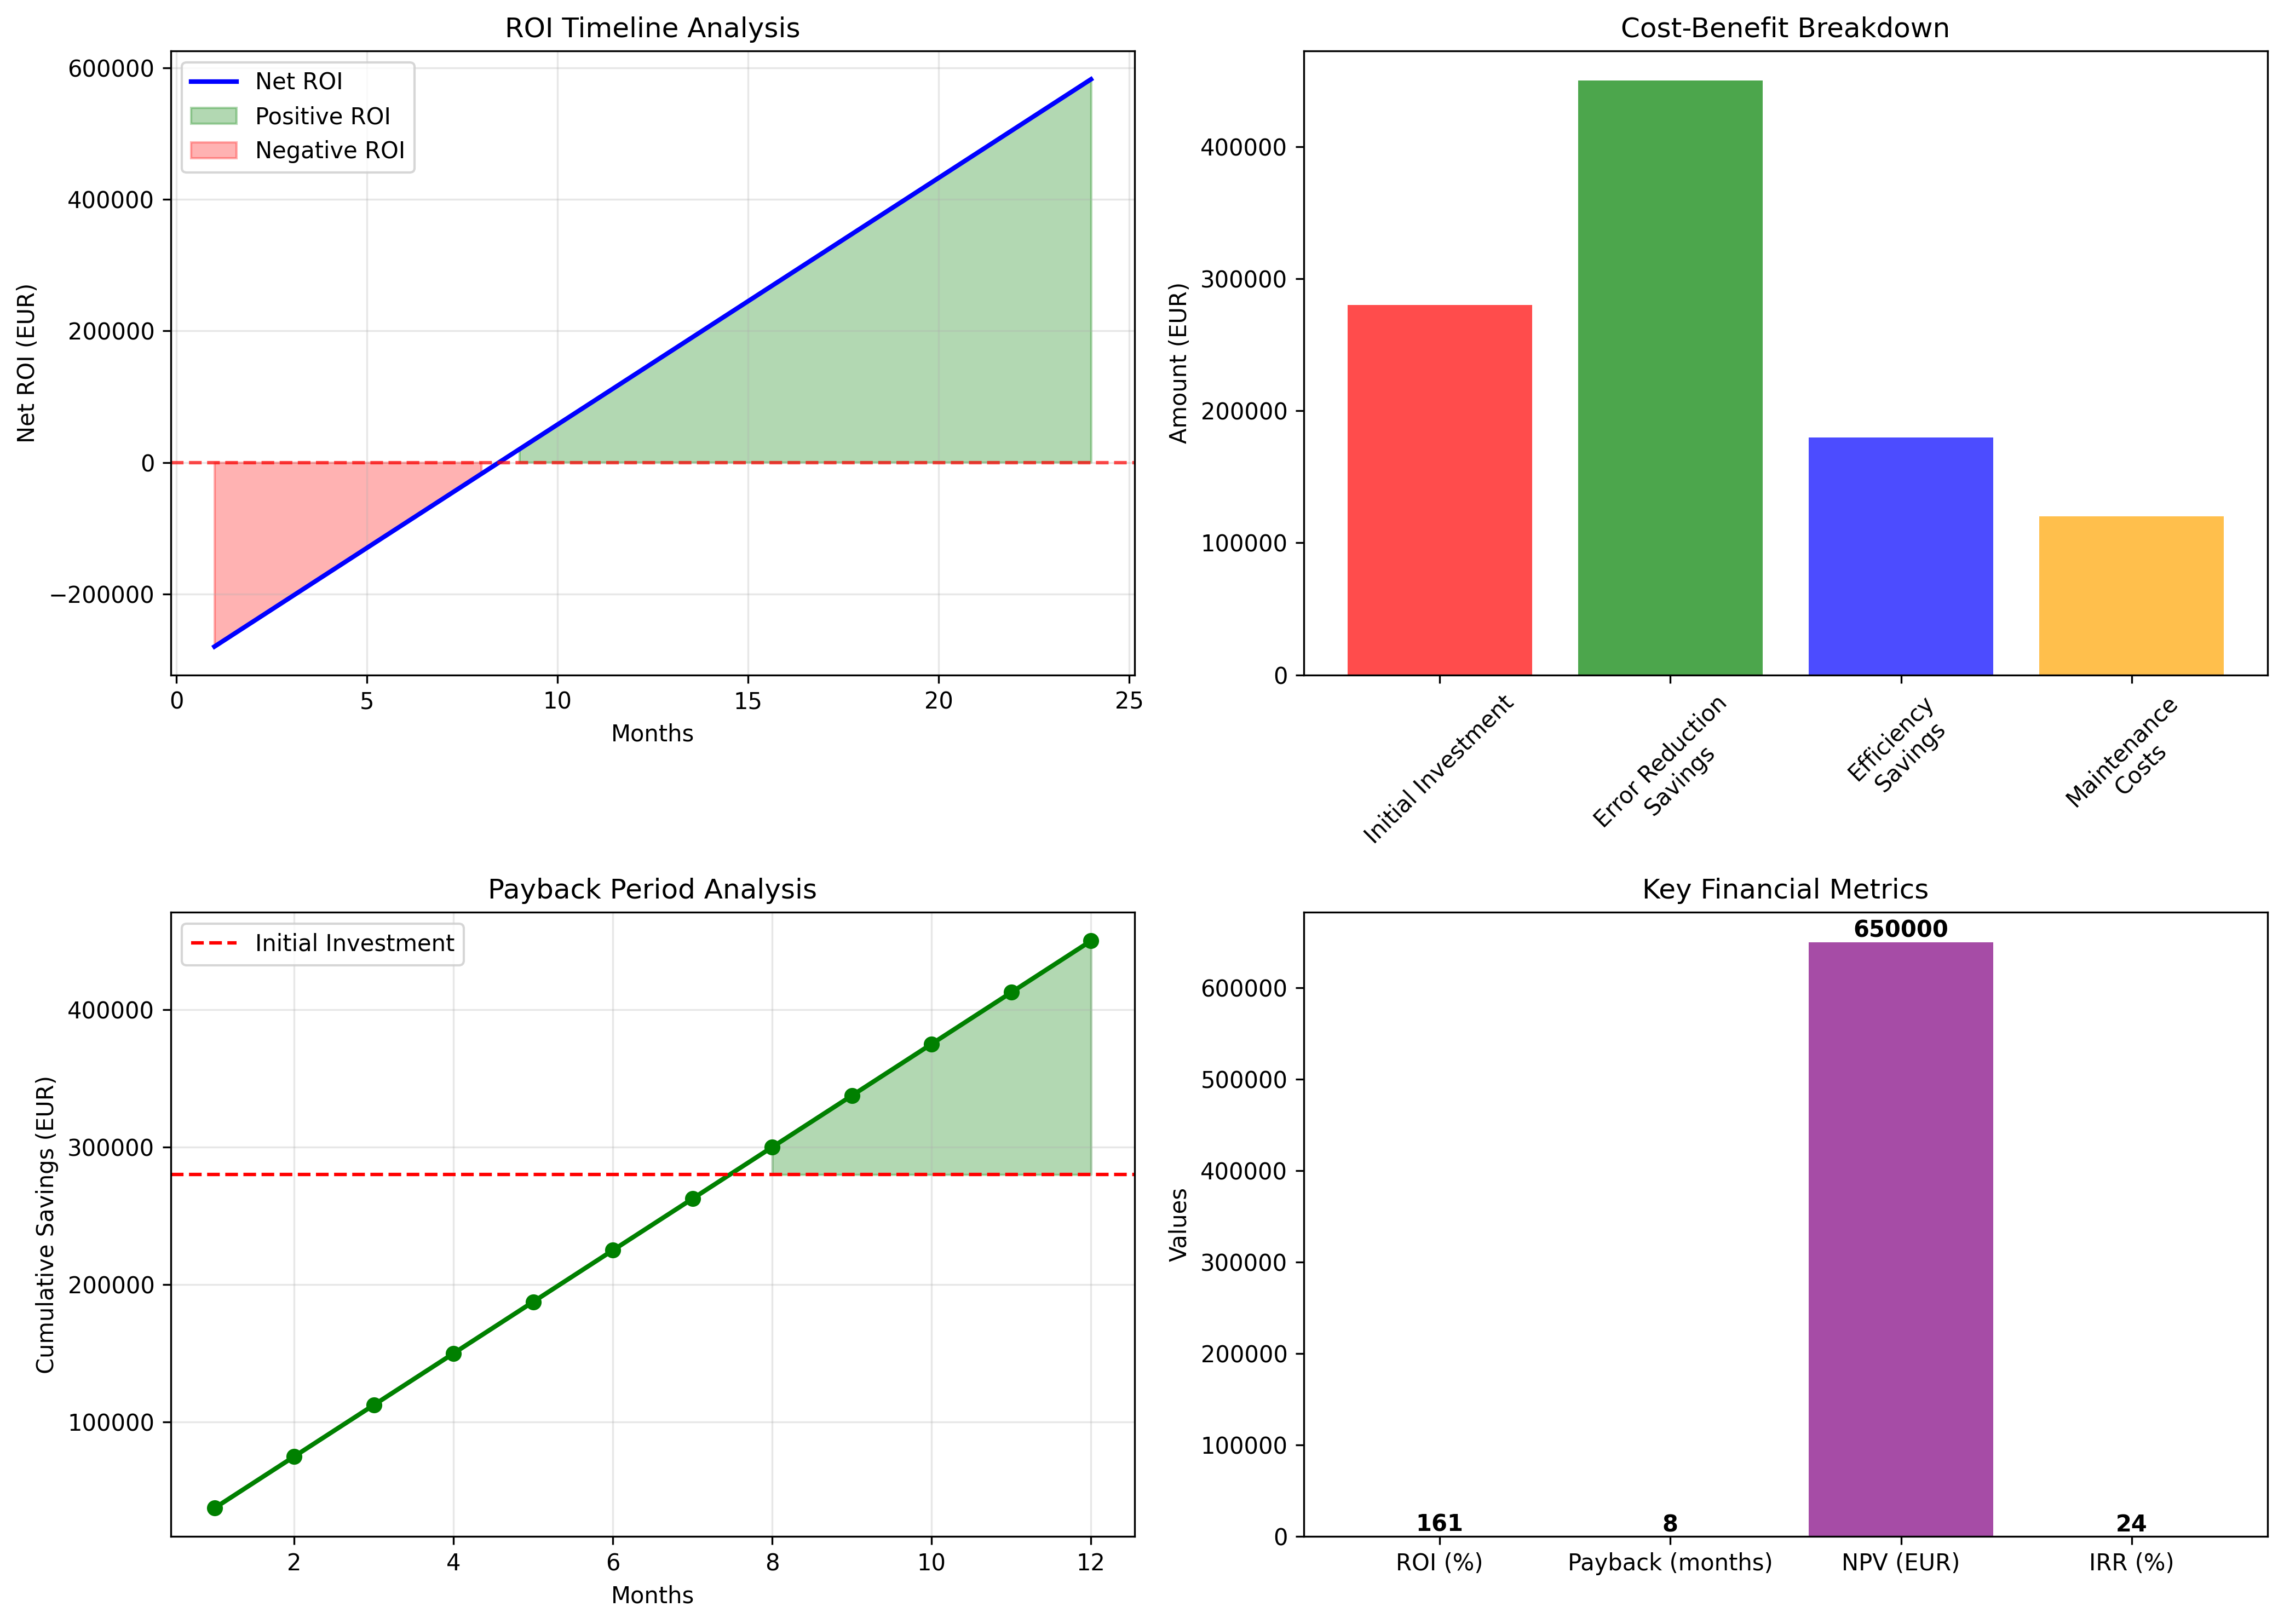
\includegraphics[width=0.95\textwidth]{images/generated/roi_analysis.png}
    \caption{Cost-benefit analysis, including investment breakdown, ROI timeline, and payback period calculation.}
    \label{fig:roi-analysis}
\end{figure}

\section{Future Development Roadmap}

The future development roadmap, outlined in Figure~\ref{fig:future-roadmap}, is structured in sequential phases over 18 months. Key initiatives include implementing AI/ML algorithms for predictive interaction analysis, achieving full HL7 FHIR compliance for enhanced interoperability, developing a native mobile application, and deploying advanced analytics dashboards.

\begin{figure}[htbp]
    \centering
    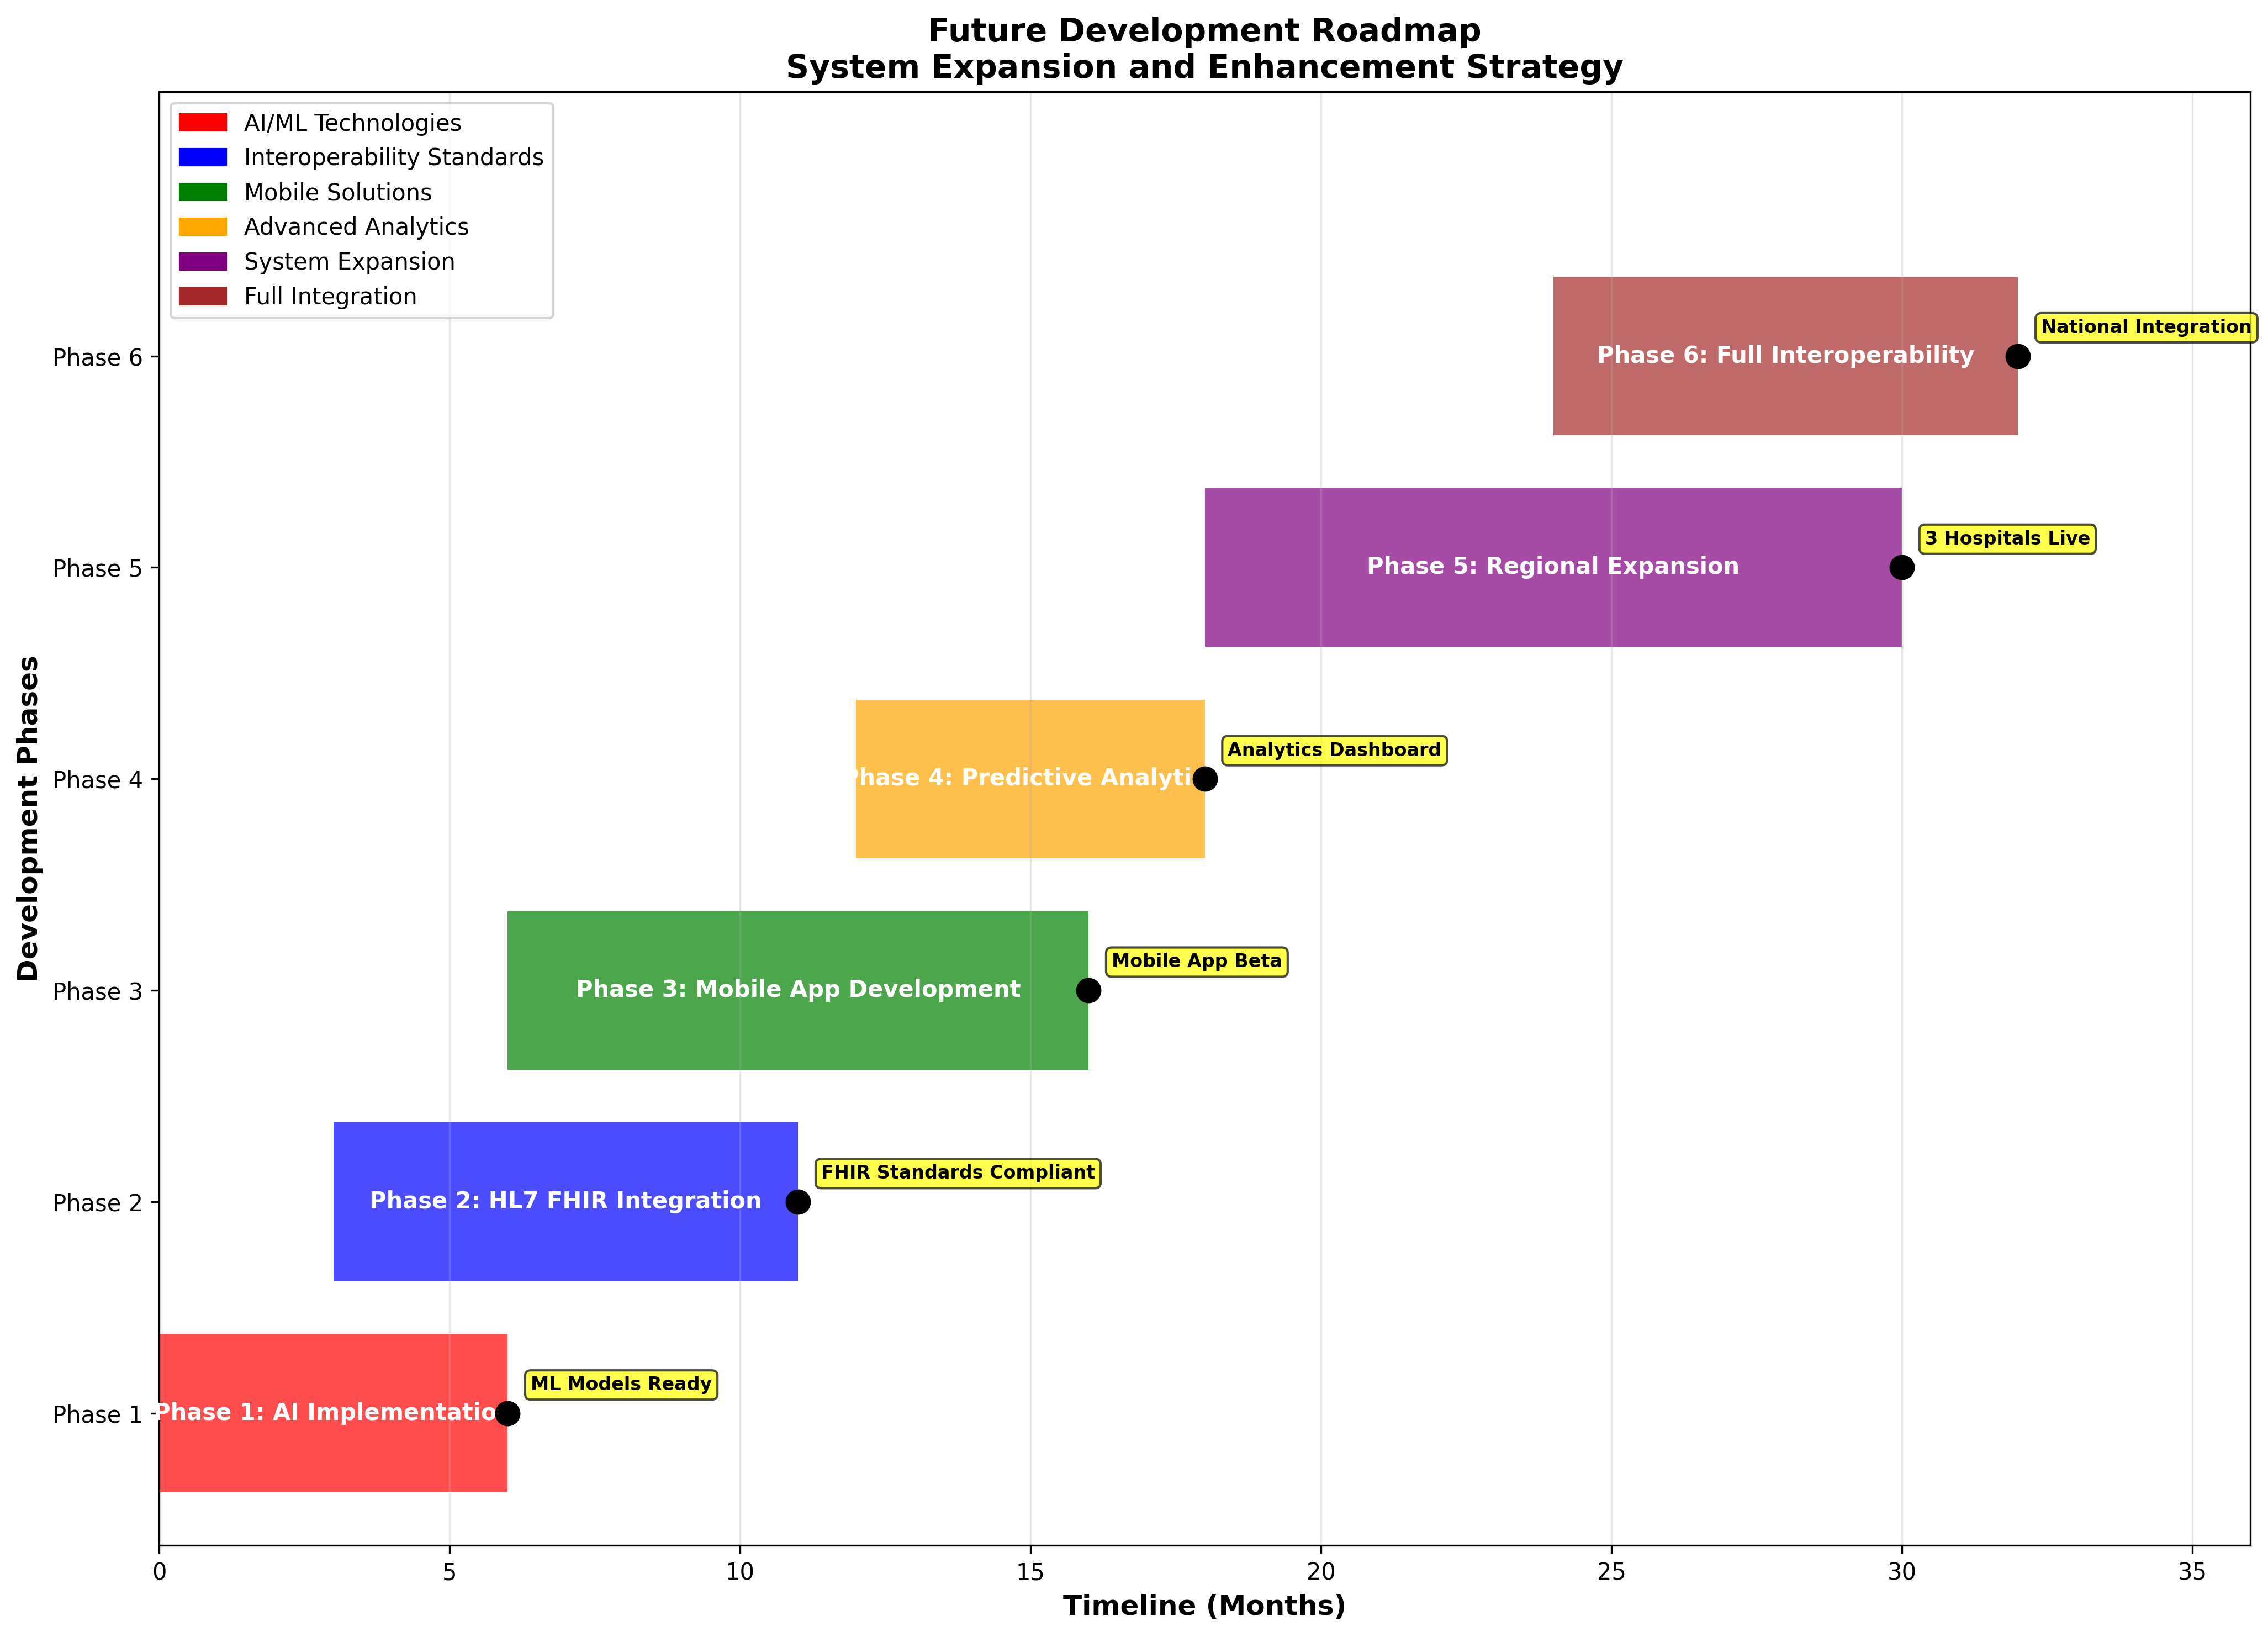
\includegraphics[width=0.95\textwidth]{images/generated/future_roadmap.png}
    \caption{18-month future development roadmap, including AI/ML features, FHIR integration, mobile application development, and regional expansion.}
    \label{fig:future-roadmap}
\end{figure}

These results demonstrate that the developed system successfully met its objectives, significantly improving patient safety, operational efficiency, and user satisfaction, thereby justifying the investment and supporting its future expansion. 